%% LaTeX-Beamer template for KIT design
%% by Erik Burger, Christian Hammer
%% title picture by Klaus Krogmann
%%
%% version 2.0
%%
%% mostly compatible to KIT corporate design v2.0
%% http://intranet.kit.edu/gestaltungsrichtlinien.php
%%
%% Problems, bugs and comments to
%% burger@kit.edu

\documentclass[18pt]{beamer}
\usetheme{kit}

%% TITLE PICTURE

% if a custom picture is to be used on the title page, copy it into the 'logos'
% directory, in the line below, replace 'mypicture' with the 
% filename (without extension) and uncomment the following line
% (picture proportions: 63 : 20, *.eps format if you use latex+dvips+ps2pdf,
% *.jpg/*.png/*.pdf if you use pdflatex)

%\titleimage{mypicture}

%% TITLE LOGO

% for a custom logo on the front page, copy your file into the 'logos'
% directory, insert the filename in the line below and uncomment it

%\titlelogo{mylogo}

% (*.eps format if you use latex+dvips+ps2pdf,
% *.jpg/*.png/*.pdf if you use pdflatex)

%% BIBTEX ICON/KEY

% if you want to see BibTeX keys in the references view instead of the symbol,
% uncomment the following line
% \usebibitemtemplate{\insertbiblabel}

% the presentation starts here

% change the following line to "ngerman" for German style date and logos
% change the following line to "english" for English style date and logos
\selectlanguage{ngerman}

\beamertemplatenavigationsymbolsempty

\usepackage{listings}
\definecolor{darkgray}{rgb}{0.95,0.95,0.95}
\definecolor{darkgreen}{rgb}{0.05,0.7,0.05}
\lstset{ language=Java,
	backgroundcolor=\color{darkgray}, 
	numbers=none, 
	keywordstyle=\color{black}\bfseries,
	tabsize=2,
	showspaces=false,               % show spaces adding particular underscores
	showstringspaces=false,         % underline spaces within strings
	showtabs=false, 
}



\title[Tutorium01]{Tutorium 02: UML in Aktion}
\subtitle{Softwaretechnik im SS 2011, Tutorien 4 + 11 + 17}
\author{Jürgen Walter}
\date{\today}

\institute{Chair for Software Design and Quality}

\begin{document}

%title page
\begin{frame}
\titlepage
\end{frame}

%table of contents
\frame{
\frametitle{Was machen wir heute?}
\tableofcontents
}

\section{Altes Übungsblatt}

\subsection{Altes Übungsblatt}
\frame {
\frametitle{Altes Übungsblatt}
\begin{block}{Aufgabe 1: Klassendiagramm}
\begin{itemize}
\item Von Hand Zeichnen!
\item Attributname : Attributtyp, nicht umgekehrt
\item Vererbungspfeile sind nicht ausgemalt\dots
\end{itemize}
\end{block}


\begin{block}{Aufgabe 2: Anwendungsfalldiagramm}
\begin{itemize}
\item Von Hand Zeichnen!
\item Alles muss zum Endknoten verbunden werden!
\item Die meissten haben nur die Hälfte der Aufgabe gelöst! 
\end{itemize}
\end{block}
}

\frame{
\begin{block}{Aufgabe 3 Floyd-Steinberg-Algorithmus} 
\begin{itemize}
\item Checkstyle: “Utility classes should not have a public or default constructor” \pause
\item Lösung: \lstinline[language=Java]"private Klassenname() \{\}"
\end{itemize}
\end{block}
}

\subsection{Zum Aufwärmen ...}
\frame {
\frametitle{Wahr oder falsch?}
\begin{itemize}
	\color<2->[rgb]{1,0,0}
	\item Das einzige Ziel der Softwaretechnik ist, die Kosten der Erstellung von Software möglichst weitgehend zu senken.
	\color[rgb]{0,0,0}
	\pause
	\color<3->[rgb]{0,1,0}
	\item UML-Anwendungsfalldiagramme werden während der Planungsphase verwendet, um das von außen sichtbare Verhalten des Systems darzustellen.
	\color[rgb]{0,0,0}
	
	\pause
	\color<4->[rgb]{0,1,0}
	\item Komposition ist eine strengere Aggregation, bei der die Teile keine Daseinsberechtigung ohne das Ganze haben.
	\color[rgb]{0,0,0}
	\pause
	\color<5->[rgb]{1,0,0}
	\item Grundsatz der Vererbung: Mache eine Klasse A erst dann zu einer Unterklasse einer Klasse B, wenn 			sicher ist, dass jede Instanz von B auch als Instanz von A gesehen werden kann.
	\color[rgb]{0,0,0}
	\pause
	\color<6->[rgb]{0,1,0}
	\item Kontravariante Eingabe-Parameter erfüllen das Substitutionsprinzip.
	\color[rgb]{0,0,0}
	\pause
	\color<7->[rgb]{0,1,0}
	\item Ein Pflichtenheft spezifiziert die Anforderungen an eine Software in eindeutiger Weise, so dass sie implementiert werden können
	\color[rgb]{0,0,0}
\end{itemize}
}

\subsection{Swing}

\frame{
\frametitle{Swing Tipps}
\begin{block}{Layouts}
\begin{itemize}
\item um Swing Komponenten anzuordnen verwendet man Layouts \pause
\item es gibt sehr viele Varianten: \url{http://download.oracle.com/javase/tutorial/uiswing/layout/visual.html}  \pause
\item für ÜB3 habt ihr freie Wahl, daher bieten sich \texttt{FlowLayout} oder ein vertikales \texttt{BoxLayout} an \pause
\item für bessere Strukturierung: gruppiert mehrere Komponenten mit einem JPanel  \pause
\item jeder Swing Container kann sein eigenes Layout haben \pause
\item default: JFrame - \texttt{BorderLayout}, JPanel -  \texttt{FlowLayout})
\end{itemize}
\end{block}
}
\begin{frame}[fragile]
\frametitle{Swing Tipps}
\begin{block}{Bilder anzeigen}
\begin{itemize}
\item grundsätzlich kann man auf jede Swing Komponente malen \pause
\item am einfachsten: \texttt{Icon} setzen \\
\url{http://download.oracle.com/javase/tutorial/uiswing/components/icon.html}  \pause
\end{itemize}
\end{block}

\begin{block}{Beispiel}
\begin{lstlisting}
	JFrame f = new JFrame();
	f.add(new JLabel(new ImageIcon(image)));
	f.setSize(200,200);
	f.setVisible(true);
\end{lstlisting}
\end{block}
\end{frame}

\begin{frame}[fragile]
\frametitle{Swing Tipps}
\begin{block}{Beispiel}
\begin{lstlisting}
			JFrame f  = new JFrame();
			f.setLayout(new FlowLayout());
			f.setSize(220,325);
			for (int i=0; i<20; i++) {
				f.add(new JLabel("Text"));
				f.add(new JButton("Button"));
			}
			f.setVisible(true);
\end{lstlisting}
\end{block}
\end{frame}


\frame {
\begin{exampleblock}{Beispiel Zustandsdiagramm}
\begin{center}
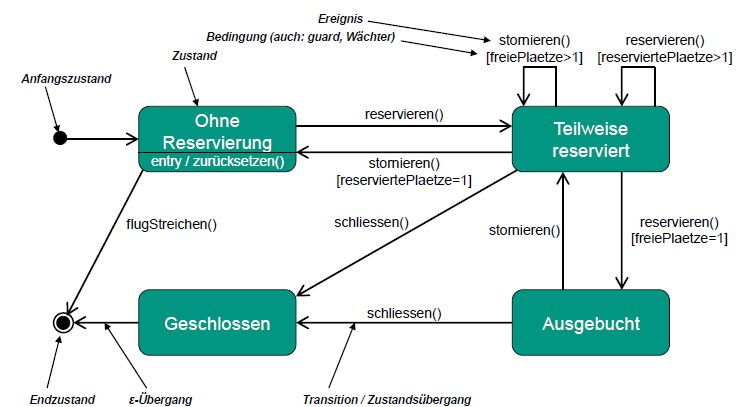
\includegraphics[scale=0.6]{pics/zustandsdiagramm.png}
\end{center}
\end{exampleblock}
}

\section{UML}

\subsection{Zustandsdiagramm}

\frame{
\frametitle {Zustandsdiagramm} 
\begin{itemize}
 \item Beschreibt mögliche Zustände eines Objekts sowie mögliche Zustandsübergänge
 \item Zustandsübergang (Transition) wird durch ein Ereignis ausgelöst
 \begin{center}
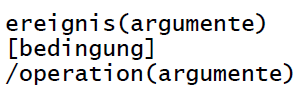
\includegraphics[scale=0.5]{pics/zustandsuebergang.png}
\end{center}
\item Zustandsübergang findet nur statt, wenn zu diesem Zeitpunkt die Bedingung erfüllt ist
\item $\epsilon$ -Übergang
\item Aktionen
\end{itemize}
}

\frame {
\begin{exampleblock}{Beispiel Zustandsdiagramm}
\begin{center}
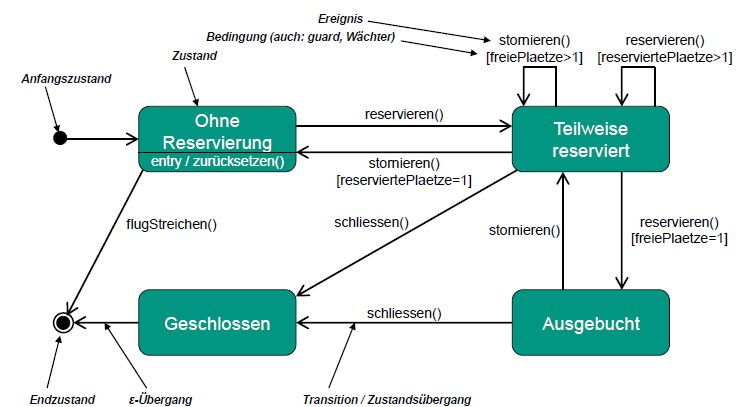
\includegraphics[scale=0.52]{pics/zustandsdiagramm.png}
\end{center}
\end{exampleblock}
}

\frame{
\frametitle {Zustandsdiagramm Aufgabe Klausur 2010 (3P)}
Wandeln Sie den rechts abgebildeten UML-Zustandsautomaten durch Zusammenlegen der Zustände $A_B$ 
und $A_C$ zu einem neuen Zustand A in einen äquivalenten hierarchischen Zustandsautomaten um. (3 P)

Hinweis: Beachten Sie, dass die gleiche Eingabefolge in Ihrem transformierten Automaten zu einem
äquivalenten Zustand führt, wie im Originalautomaten (z. B.: Start $\rightarrow$ 1, 2, 3, 1 $\rightarrow$ C).
\begin{center}
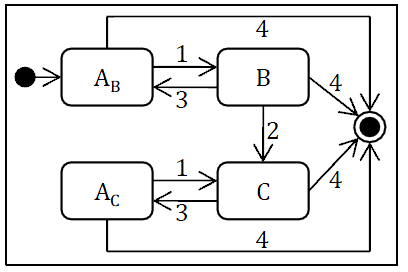
\includegraphics[scale=0.5]{pics/ZustandsdiagrammAufgabe.png}
\end{center}
}

\frame {
\frametitle {Musterlösung} 
\begin{center}
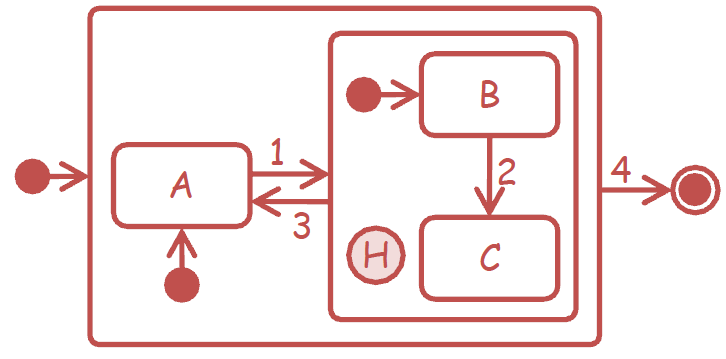
\includegraphics[scale=0.6]{pics/MZustandsdiagrammAufgabe.png}
\end{center}
}

\subsection{Sequenzdiagramm}
\frame {
\frametitle {Sequenzdiagramm}
\begin{block}{Sequenzdiagramm - Wie verschicke ich Nachrichten?}
\begin{center}
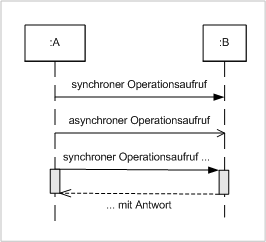
\includegraphics[width=0.6\textwidth]{pics/SequenzDiagramm1}
\end{center}
\end{block}

}

\frame {
\frametitle {Aufgabe Sequenzdiagramm 2010 (5P)}
\small {
Ein Passagierjet p meldet seinen momentanen Kurs $k_p$ an den Kontrollturm. Der Kontrollturm beauftragt den nächsten freien Fluglotsen f zu berechnen, ob irgendwelche Flugobjekte ausweichen müssen. Der Fluglotse kommt zu dem Ergebnis, dass keine Kol-lisionsgefahr besteht und alle Flugobjekte ihren Kurs beibehalten können. Folglich antwortet er mit einem leeren Feld von Kursen. Anschließend meldet ein Helikopter h sei-nen Kurs $k_h$ an den Kontrollturm. Wieder ist der nächste verfügbare Fluglotse der Flug-lotse f. Dieser berechnet unter Berücksichtigung von $k_h$, ob nun Flugobjekte ausweichen müssen. Diesmal besteht eine Kollisionsgefahr zwischen dem Passagierjet und dem Helikopter. Deswegen antwortet der Fluglotse mit zwei Ausweichkursen $k’_p$ und $k’_h$ für den Passagierjet bzw. den Helikopter. Der Kontrollturm weist daraufhin den Passagierjet und den Helikopter an ihre Kurse auf den jeweiligen Ausweichkurs zu ändern.
\\
Hinweis: Modellieren Sie die Kurse nicht als Objekte mit Lebenslinie. Wenn Sie Kurse als Parameter/Rückgabewert benötigen, verwenden Sie die vorgegebenen Bezeichner aus dem Szenario. Zeichnen Sie zu jedem Methodenaufruf auch die Rückantwort ein
}
}

\frame {
\frametitle {Musterlösung} 
\begin{center}
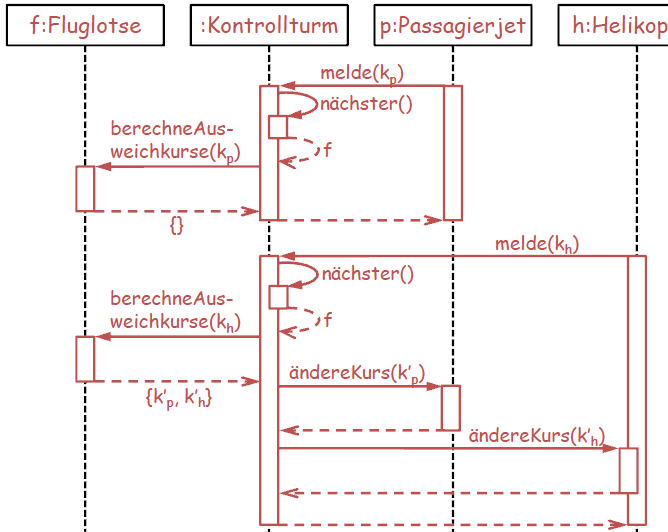
\includegraphics[scale=0.5]{pics/MSequenzdiagrammAufgabe.png}
\end{center}


}

\section{Ende}

\subsection{Tipps zum nächsten Übungsblatt}

\frame{
\frametitle{Tipps zum nächsten Übungsblatt}

\begin{block}{Aufgabe 1 - Sequenzdiagramm}
\begin{itemize}
\item denkt an Lebenslinien, synchrone vs. asynchrone Nachrichten, Steuerungsfokus \pause
\item laut Folien sind Fokus und Antworten egal, können aber in Klausur gefordert sein \pause
\item zeichnet sie also am Besten immer ein
\end{itemize}
\end{block}

\begin{block}{Aufgabe 2 - Zustandsdiagramm}
\begin{itemize} \pause
\item gebt stets das “Gedächtnis”' des Diagramms mit an
\end{itemize}
\end{block}

}


\frame{
\frametitle{Tipps zum nächsten Übungsblatt}
\begin{block}{Aufgabe 3 - Programmieren}
\begin{itemize}
\item besteht aus den Teilaufgaben “GUI” und Floyd-Steinberg für 3,6,..,24-Bit RGB \pause
\item denkt an
\texttt{int p = (o + 128 ) / 256 * 255 }
\\ hier müsst ihr ansetzen um von 256 möglichen Ergebnissen auf $2^i$ mögliche Ergebnisse zu reduzieren \pause
\item für das GUI gibt es unzählige Tutorials u.a. bei Oracle:
\\ \url{http://download.oracle.com/javase/tutorial/uiswing/components/index.html}
\\ \url{http://download.oracle.com/javase/tutorial/uiswing/components/componentlist.html}
\\ \url{http://download.oracle.com/javase/tutorial/uiswing/layout/visual.html}
\end{itemize}
\end{block}
}

\frame{
\frametitle{Tipps zum nächsten Übungsblatt}
\begin{block}{Bonusaufgabe - Klassendiagramm}
\begin{itemize}
\item gute Übungsmöglichkeit
\item für alle deren Klassendiagramme nicht fehlerfrei waren ;)\pause
\item zeichnet die Diagramme von Hand: \\
 in der Klausur hilft euch auch keine Software
\end{itemize}
\end{block}
}


\frame{
\frametitle{Bis zum nächsten Mal}
\begin{center}
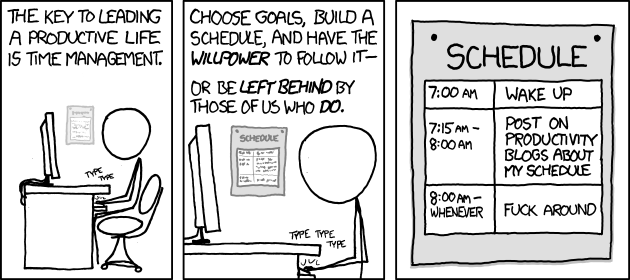
\includegraphics[width=1\textwidth]{pics/time_management}
\end{center}

}


\end{document}
